\item
\mbox{}
\begin{center}
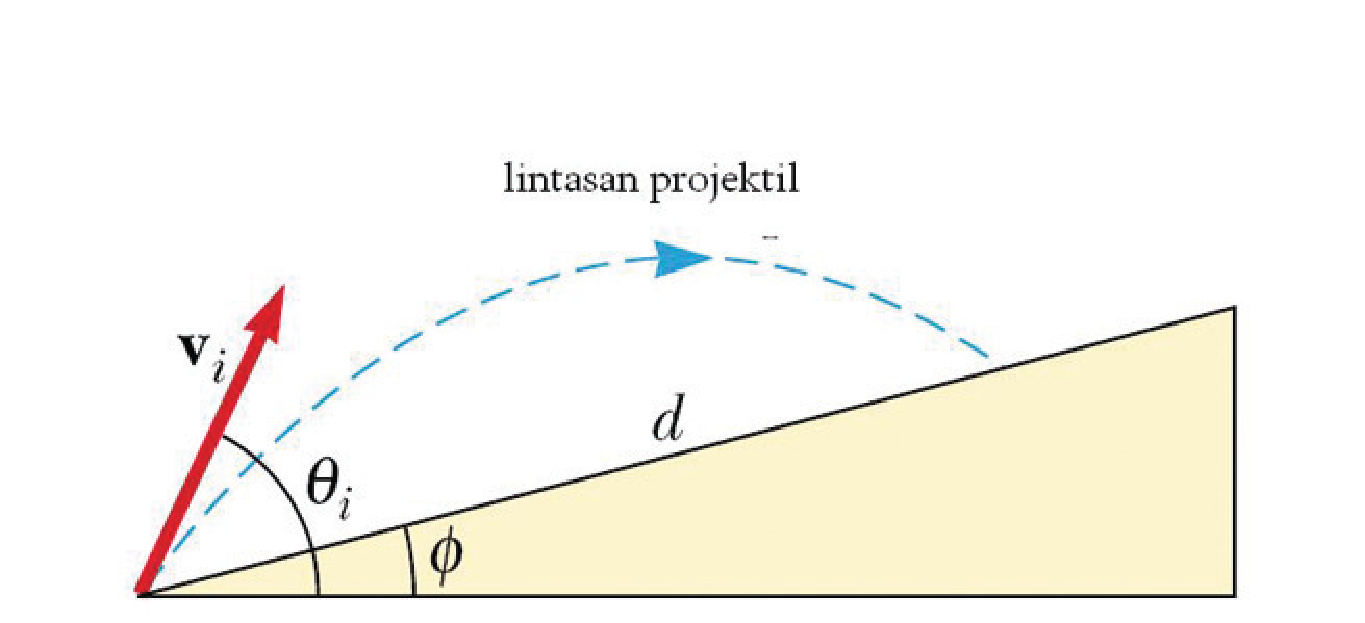
\includegraphics [scale=0.3]{./latex/eps/1_4_1_image_1-eps-converted-to.pdf}
\end{center}a. Projektil dilontarkan pada bidang miring dengan sudut $\phi$ dengan kecepatan awal $v$ dan sudut $\theta$ terhadap horizontal seperti pada gambar. Tunjukan bahwa projektil akan menempuh jarak $d$, dimana $d$ =
\begin{equation*}
        d= \frac{2 v \cos \left(\theta\right) \sin\left(\theta-\phi\right)}{g \cos^2\left(\theta\right)}
\end{equation*}

b. Berapa nilai $\theta$ supaya $d$ maksimum dan berapa nilai maksimum tersebut ?
\begin{description}
\item[Solusi:]
a. bila projektil menyentuh bidang miring pada jarak $d$ maka, \\ \\$x_{f}=d \cos\left(\phi\right)$ dan $y_{f}=d \sin\left(\phi\right)$ (subscript f artinya final). \\ \\
Bila hal tersebut terjadi pada waktu $t$, maka \\ \\ $t=\frac{x_{f}}{v \cos\left(\theta\right)}$ dan $y_{f}=v \sin\left(\theta\right) t-\frac{1}{2}g t^{2}$ \\ \\
dengan mensubstitusi $t$ ke dalam $y_{f}$, didapat \\ \\
$y_{f}=\tan\left(\theta\right) x_{f}-\frac{g }{2 \cos^{2} \theta}x_{f}^{2}  $\\ \\
Kemudian mensubsitusi nilai $x_{f}=d \cos\left(\phi\right)$ dan $y_{f}=d \sin\left(\phi\right)$, menjadi, \\ \\
\begin{eqnarray*}
d \sin \phi &=& \tan\left(\theta\right) d \cos-\frac{g }{2 v^{2} \cos^{2} \theta}\left(d \cos \phi\right)^{2} \\
 \sin \phi &=& \tan\left(\theta\right) \cos-\frac{g }{2 v^{2} \cos^{2} \theta} d  \cos^{2} \phi \\
 \frac{\sin \phi \cos \theta-\sin \phi \cos \theta}{\cos \theta} &=& \frac{-g}{2 v^2 \cos^2 \theta} d \cos^{2} \phi \\
 \frac{\sin \left(\phi-\theta\right)}{\cos \theta}&=& \frac{-g}{2 v^2 \cos^2 \theta} d \cos^{2} \phi \\ \\
 \mbox{jadi} \\
  d&=&\frac{2 v^2 \cos \theta \sin \left(\theta-\phi\right)}{g \cos^{2} }
\end{eqnarray*}

b. $d$ mencapai maksimum bila $\frac{d d}{d \theta}=0$
\begin{eqnarray*}
\frac{2 v^{2}}{g \cos^{2} \phi}\left[-\sin \theta \sin \left(\theta-\phi\right)+\cos \theta \cos\left(\theta-\phi\right)\right] &=& 0 \\
-\sin \theta \sin \left(\theta-\phi\right)+\cos \theta \cos\left(\theta-\phi\right) &=& 0 \\
\cos \left(\theta-\phi+\theta\right) &=& 0 \\
\cos \left(2\theta-\phi\right) &=& \cos 90^{0} \\
\theta &=& 45^{0}+\frac{\phi}{2}
\end{eqnarray*}
jadi d maksimum apabila
\begin{equation}
d_{max}=\frac{v^{2}\left(1-\sin \phi\right)}{g \cos^{2} \phi}
\end{equation}

\end{description}
